\section{Current solutions and approaches}

% Hvem gør allerede sådan noget her.
% Hvordan gør de det? Hvilke frameworks, theories,  etc. bruger de?


% Der er ingen som gør præcis som os, men et set af services ville kunne gøre det samme. 
% Google, Facebook, Snapchat
% Facebook grupper. Snapchats location stuff. Google data om venues etc.

Sharing the locations of users/locations is a popular feature in many modern systems, such as \texttt{Google} with locations and ratings of venues and \texttt{Facebook} or \texttt{Snapchat} with groupings and available locations of associates. These domains all have features resembling subsets of our main objective, but as \textit{side features} and does not satisfy the specified requirements individually \textit{or} as a whole.

\textbf{Google: }\\
\texttt{Google} offers increasingly more information for venues and events, creating both a more user friendly interface and advertisement for the respective venues or events. One can easily see previous ratings and activity levels at e.g. cafe's and bars. Google Maps also offers features such as locations of venues and current device location. 
Additionally pictures, opening hours, websites, transport directions, reviews, keywords, handicap concerns, and many other kinds of information is available through the google api. 

\textbf{Facebook: }\\
One of the main features of \texttt{Facebook} is grouping of associates, either through friendship associations or by membership of a group/project. The introduction of \texttt{Geotags}/\texttt{Geolocation} made it possible for users to post their immediate locations or 'check in' at a venue thereby share their location with their associates, but as an active action from the user.


\textbf{Snapchat: }\\
As of June 2017 \texttt{Snapchat} introduced their \textit{Snap Map} making it possible for snap chat users, to see the locations of associates. 

\vspace{1cm}
Examples of how the different domains support these features are viewed in figure \ref{fig:domains}.

\begin{figure}[H]
\centering
    \begin{subfigure}{0.32\textwidth}
    \centering
    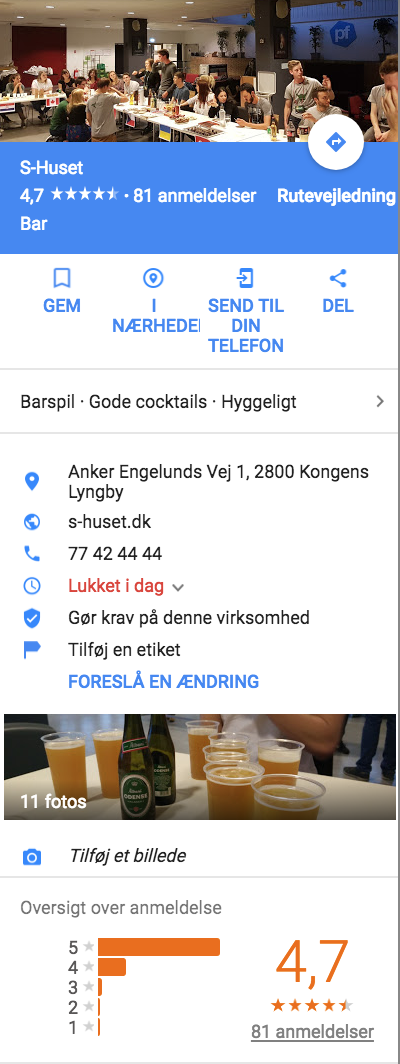
\includegraphics[width=0.8\linewidth]{images/GoogleReview.png} 
    \caption{Google review example}
    \end{subfigure}
    \begin{subfigure}{0.32\textwidth}
    \centering
    
\includegraphics[width=0.8\linewidth]{images/FacebookGroup.png} 
    \caption{Facebook group example}
    \end{subfigure}
    \begin{subfigure}{0.32\textwidth}
    \centering
    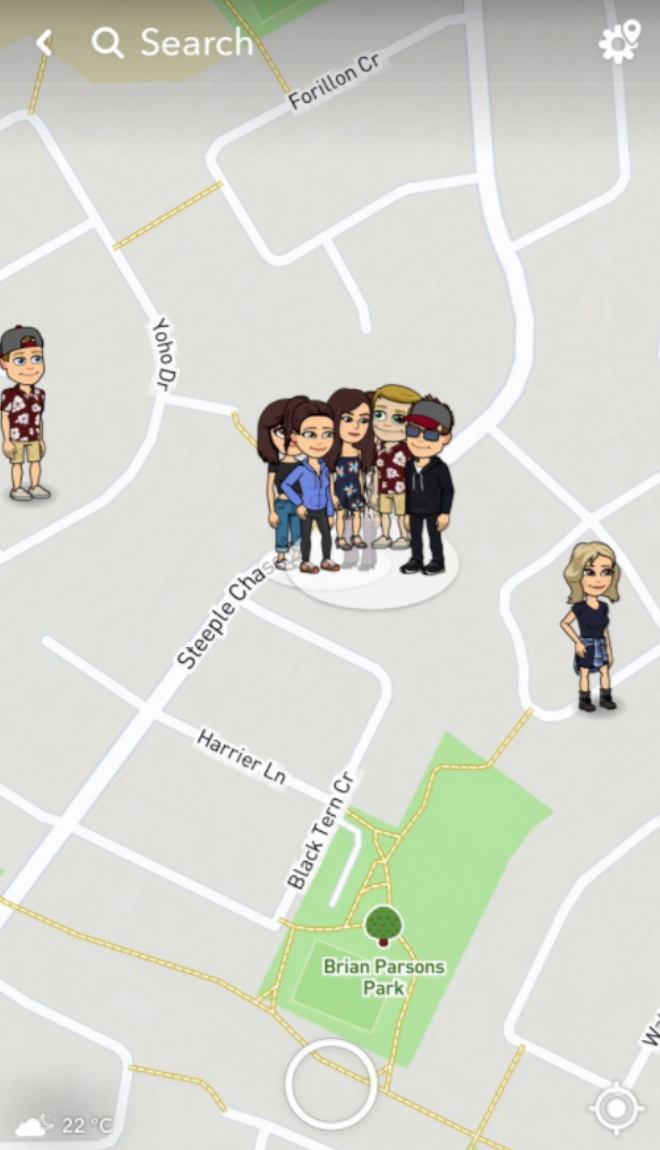
\includegraphics[width=0.8\linewidth]{images/SnapMap.png} 
    \caption{Snap Map example}
    \end{subfigure}
    \caption{Resembling domain examples}
    \label{fig:domains}
\end{figure}